\documentclass[12pt, a4paper, titlepage]{article}
\usepackage[utf8]{inputenc}
\usepackage[english]{babel}
\usepackage[T1]{fontenc}
\usepackage{enumerate}
\usepackage{graphicx}
\usepackage{hyperref}
\hypersetup{colorlinks=true, linkcolor=blue}
\title{Architectures of Intelligence \\ Assignment 5}
\author{Ramon Meffert (S2702207) \\ Robin Koning (S2998254)}
\date{\today}
\begin{document}
\maketitle
\section{Part one} % (fold)
\label{sec:part_one}
\begin{enumerate}[a.]
	% a screenshot in which you show values (right click, Value) for ensembles 
	% a, b, and c, while running your model and varying the stimulus, 
	% demonstrating the effects of the various connections that you made.
	
	\item A screenshot of the values of ensembles \textbf{a}, \textbf{b} and \textbf{c} can be found at \hyperref[fig:1a]{Figure~\ref{fig:1a}}. 
	
	Note that ensembles \textbf{a} and \textbf{b} react to changes rather quickly, while ensemble \textbf{c} adjusts more slowly. This is due to the fact that the synaptic constant is set to its default value (5ms) for the connections \emph{stimulus~$\rightarrow$~a}, \emph{a~$\rightarrow$~b} and \emph{b~$\rightarrow$~c}, whereas the connection used to create the simple memory, \emph{c~$\rightarrow$~c}, has a synaptic constant set at 100ms.
	
	% a screenshot of the tuning curves of ensemble a (right click on a,
	% Details…, Plots). Explain what those tuning curves indicate.
	\item A screenshot of the tuning curves of ensemble \textbf{a} can be found at \hyperref[fig:1b]{Figure~\ref{fig:1b}}.
	
	The tuning curves represent at which value of $x$ (the input) the neurons respond most frequently. In order to give a good representation of the input value as the output value, many neurons are tuned to different ``sections'' of the range of the input value, in a way ``specializing'' in recognizing a specific value and firing most often when their value is the input value. This means that together, the neurons will generate a value that will resemble the input value, as there are 100 neurons -- which is plenty to represent a range from -1 to 1.
	
	% Set the stimulus to 0. Explain the pattern that you see in the value
	% displays of a, b, and c.
	\item 
		\begin{itemize}
			\item Ensemble \textbf{a} has the same value as the stimulus.
			\item Ensemble \textbf{b} has a value of $-0.5$, because the connection a~$\rightarrow$~b uses the function \texttt{centered\_square(a)} which takes the value in \texttt{a} and applies the function $(a*a-0.5)$. $0*0-0.5 = 0.5$
			\item Ensemble \textbf{c} has a value of around $-1.1$. This is because the input to c remains non-zero, causing the integrator (i.e. the simple memory) to saturate quickly, meaning it will tend to its extreme value.
		\end{itemize}
\end{enumerate}
% section part_one (end)
\section{Part two} % (fold)
\label{sec:part_two}
A screenshot showing the model running from a tiger can be found at \hyperref[fig:2]{Figure~\ref{fig:2}}.
% section part_2 (end)
% figures
\begin{figure}[p]
	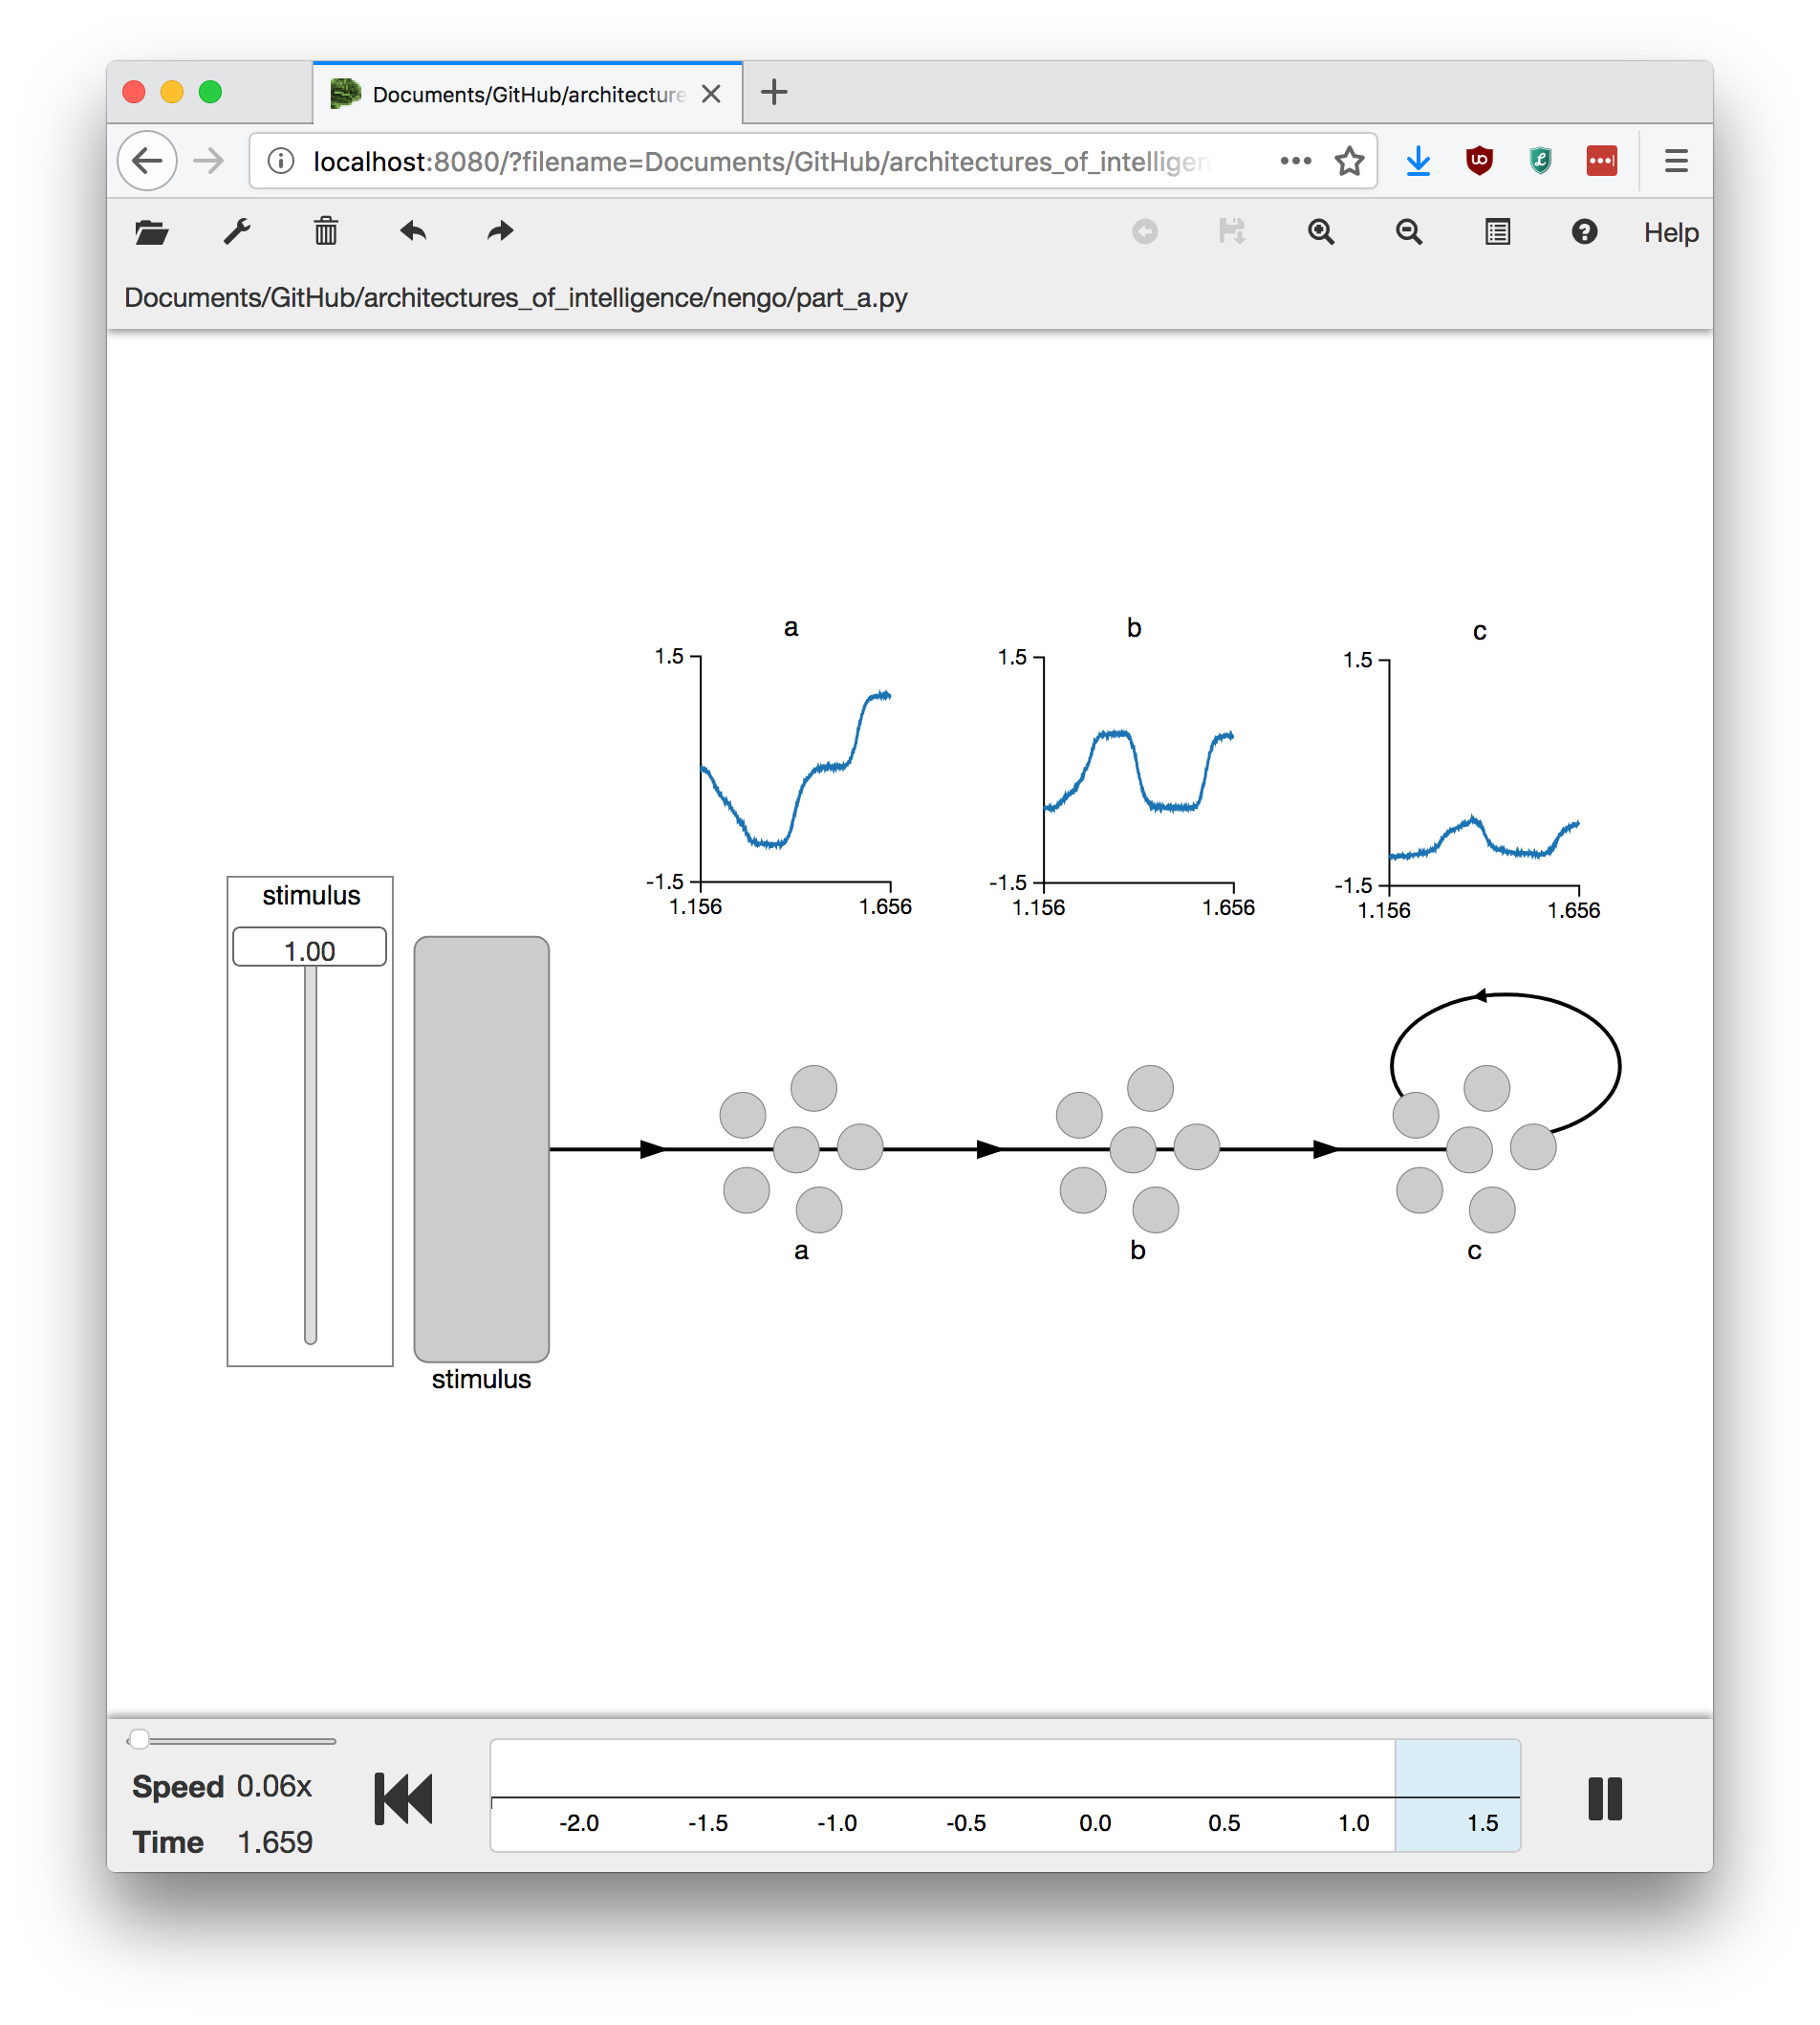
\includegraphics[width=\textwidth]{screenshot_part_1_a.png}
	\caption{Values for ensembles a, b, and c, while running the model and varying the stimulus, demonstrating the effects of the various connections}
	\label{fig:1a}
\end{figure}
\begin{figure}[p]
	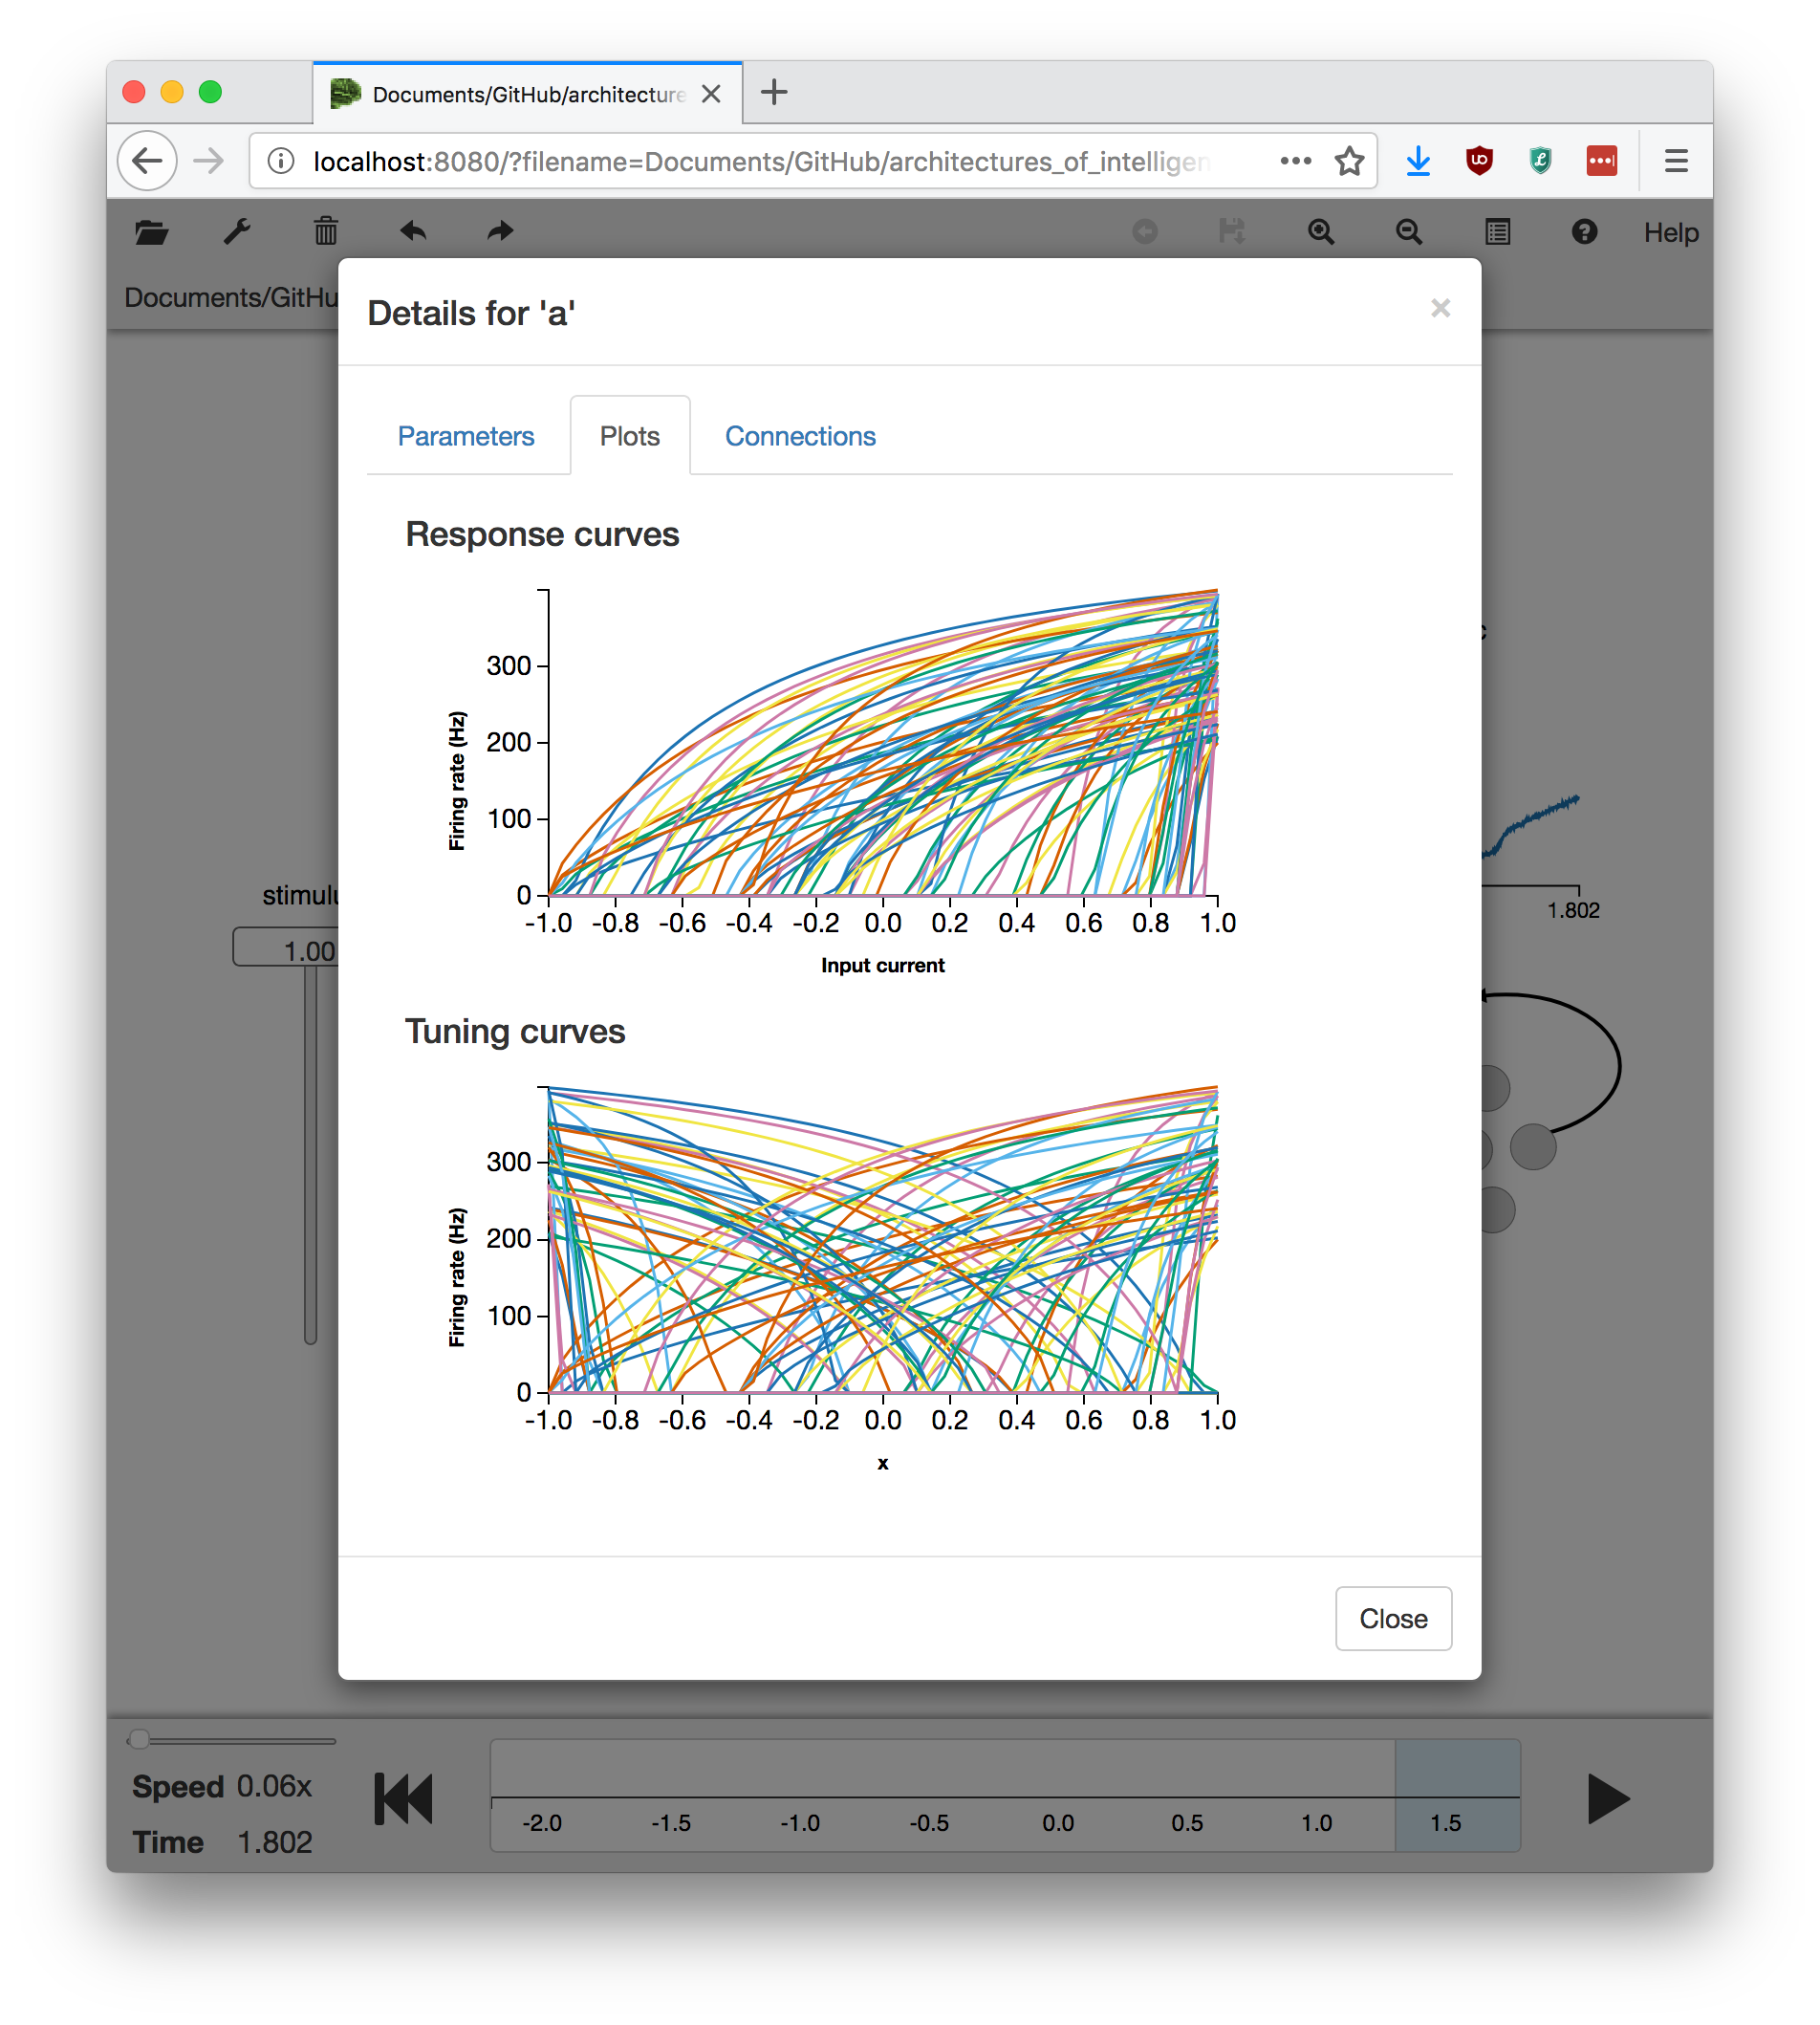
\includegraphics[width=\textwidth]{screenshot_part_1_b.png}
	\caption{A screenshot of the tuning curves of ensemble \textbf{a}}
	\label{fig:1b}
\end{figure}
\begin{figure}[p]
	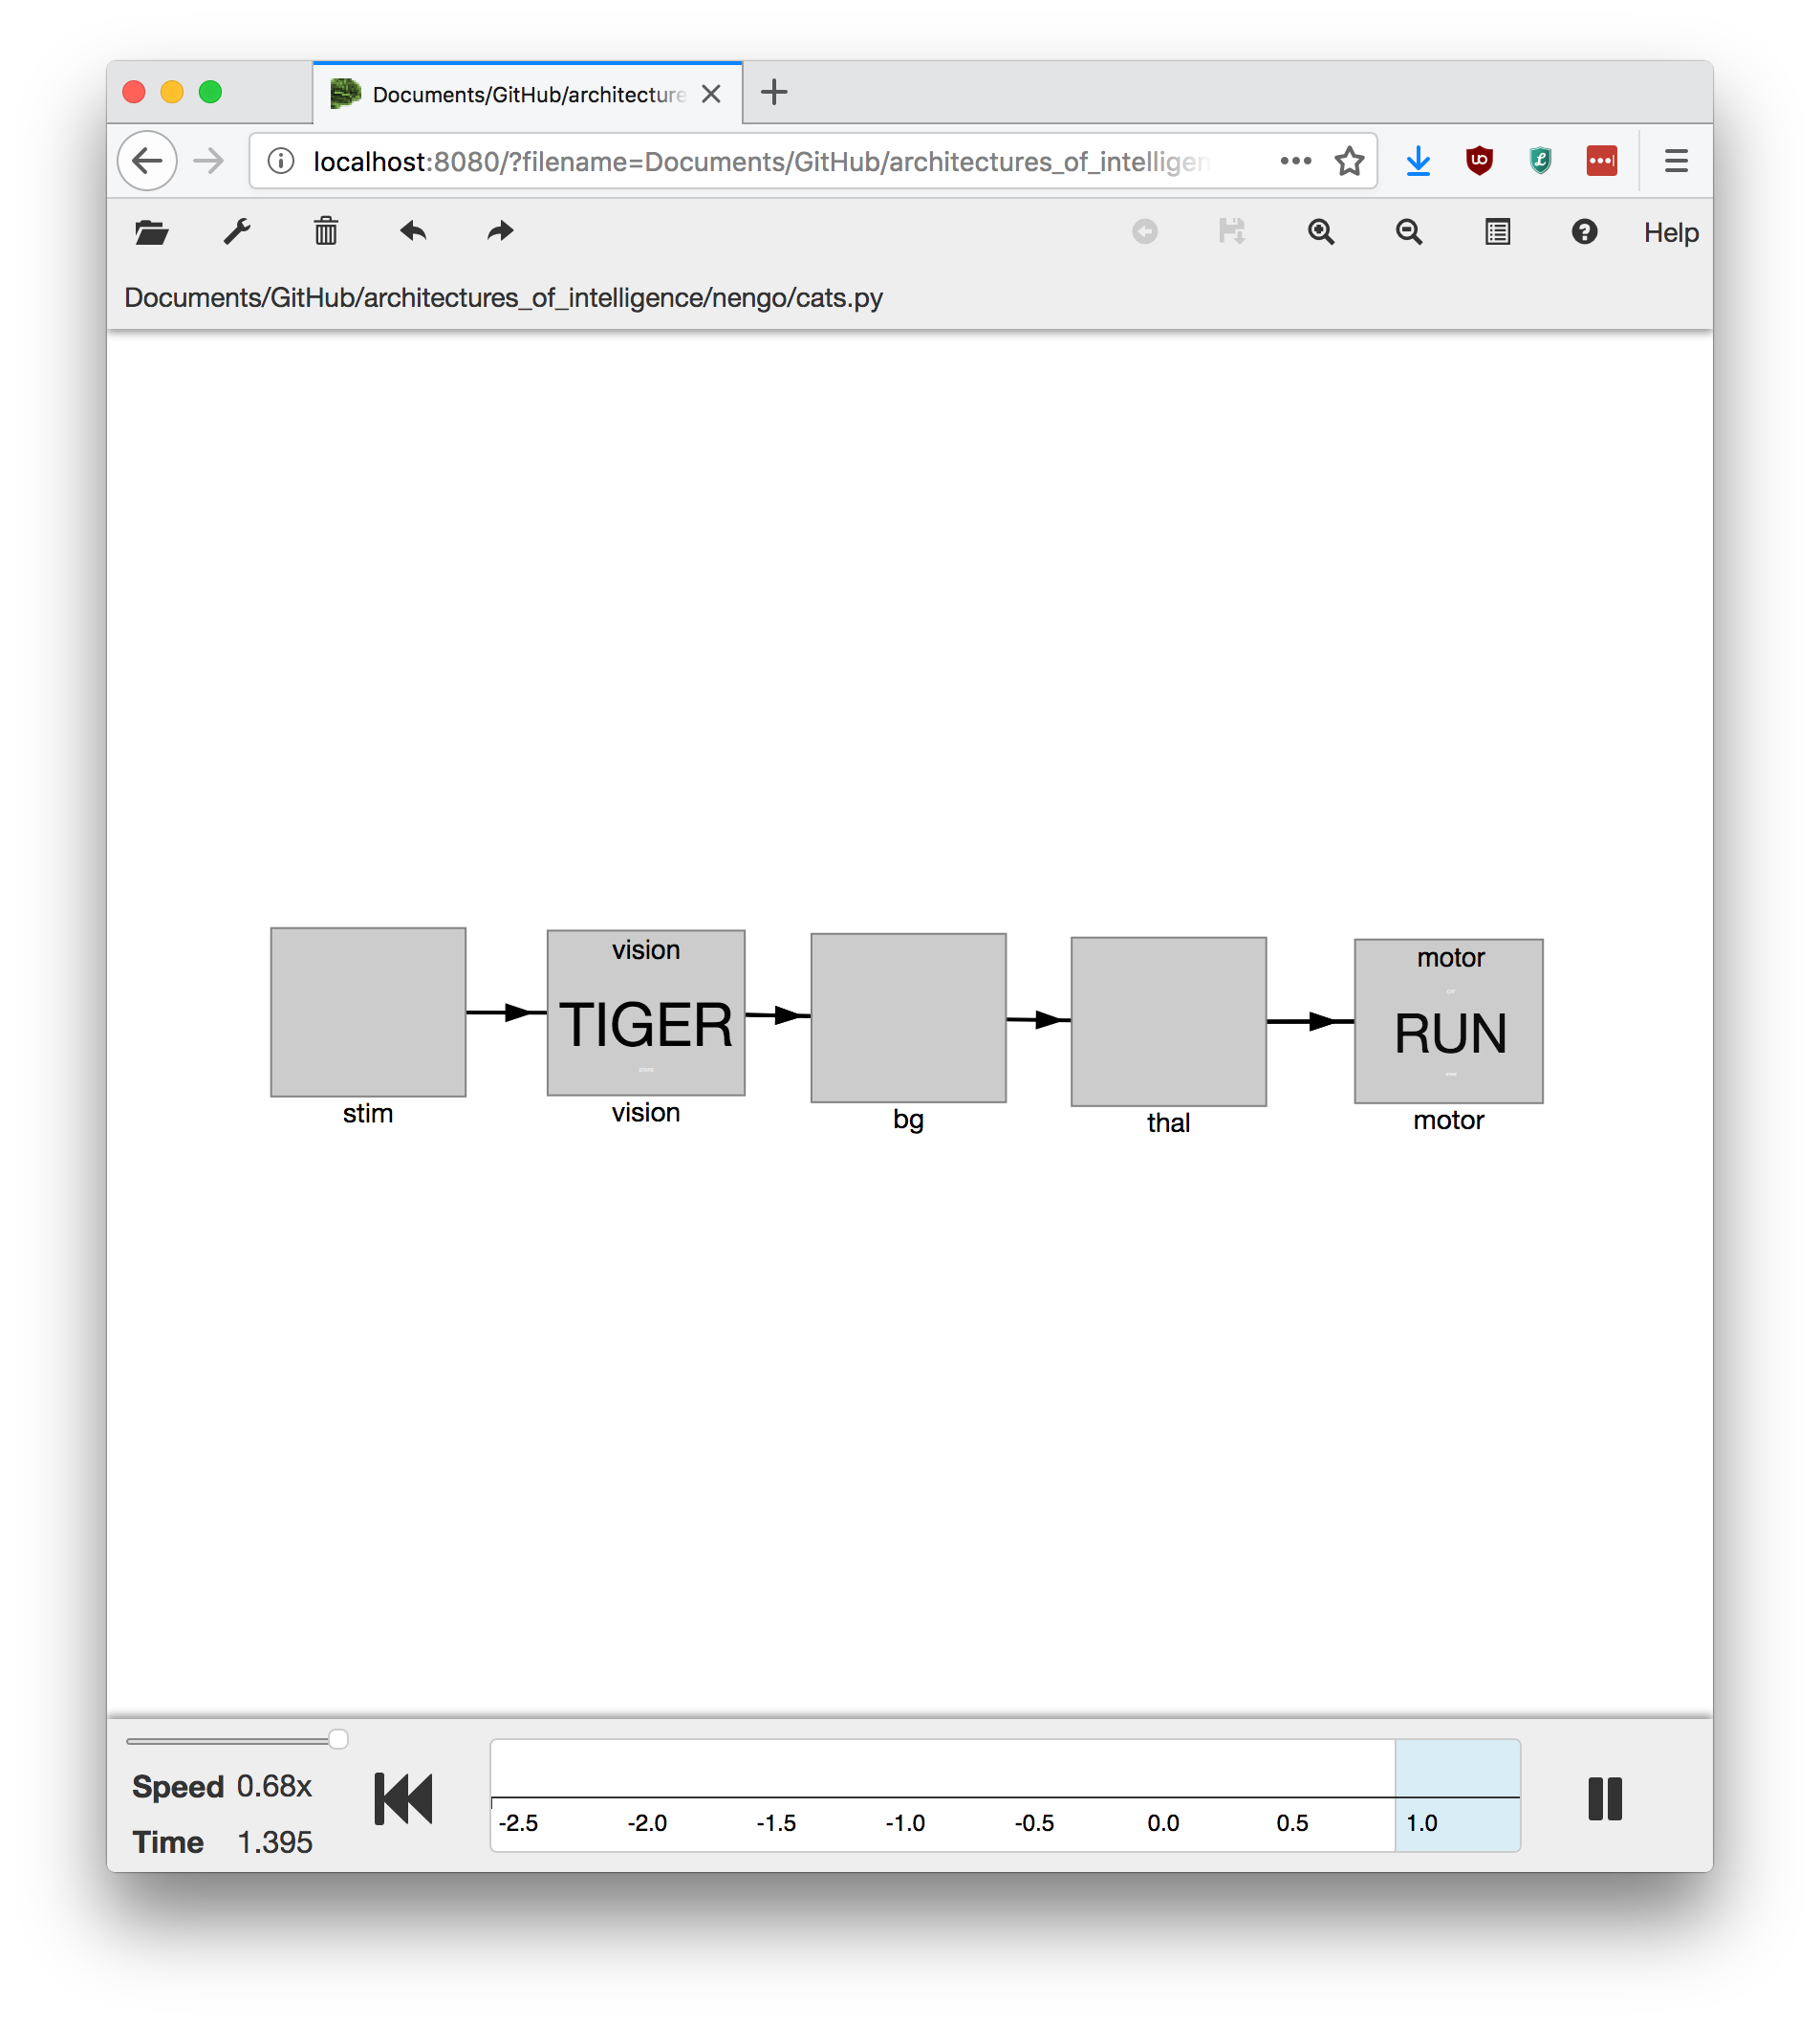
\includegraphics[width=\textwidth]{screenshot_part_2.png}
	\caption{A screenshot showing the model running from a tiger}
	\label{fig:2}
\end{figure}
\end{document}